\documentclass[11pt,a4paper]{article}

\usepackage[margin=1in]{geometry}
\usepackage[T1]{fontenc}
\usepackage{lmodern}
\usepackage{graphicx}
\usepackage{booktabs}
\usepackage{array}
\usepackage{float}
\usepackage{hyperref}
\usepackage{xcolor}
\usepackage{enumitem}
\usepackage{setspace}

\hypersetup{
    colorlinks=true,
    linkcolor=blue!60!black,
    urlcolor=blue!60!black,
    citecolor=blue!60!black
}

\setstretch{1.08}
\setlength{\parskip}{0.5em}
\setlength{\parindent}{0pt}

\title{\textbf{RepViT for CIFAR-10:}\\Architecture Adaptation, Latency-Aware Simplification, and Comparative Evaluation}
\author{Repository Analysis Report}
\date{March 28, 2026}

\begin{document}

\maketitle

\begin{abstract}
This report analyzes a CIFAR-10 adaptation of RepViT implemented in this repository. The central idea is that RepViT was originally designed around larger ImageNet-style inputs, while CIFAR-10 images are only \(32 \times 32\). Directly reusing the original early downsampling pattern causes aggressive spatial compression before the network has had enough opportunity to learn meaningful local structure. To address this, the custom \texttt{repvit\_cifar10} model reduces the patch embedding stride from \(2,2\) to \(1,1\), preserving feature-map resolution in the earliest layers. The design also removes squeeze-and-excitation (SE) blocks from the deeper stages to control inference latency, while retaining alternating SE blocks in the early stages where feature recalibration is more valuable on small inputs. Using the training and latency logs stored in the repository, the customized model achieved the best recorded CIFAR-10 accuracy (\(91.02\%\)) while maintaining latency nearly identical to the baseline RepViT-m1.1 variant.
\end{abstract}

\section{Introduction}

The repository implements and evaluates a custom RepViT variant targeted at CIFAR-10 classification. The project compares three models:
\begin{itemize}[leftmargin=1.5em]
    \item the baseline \texttt{repvit\_m1\_1},
    \item a modified \texttt{repvit\_cifar10}, and
    \item \texttt{mobilenetv3\_large\_100} as an efficient convolutional baseline.
\end{itemize}

The main engineering question is whether RepViT can be adjusted to better suit very small images without giving up its efficiency-oriented design. The answer proposed by this codebase is not to make the network larger, but to make its early feature extraction less destructive and its deeper attention-like calibration lighter.

\section{Repository Overview}

The repository organizes the project in a straightforward way:
\begin{itemize}[leftmargin=1.5em]
    \item \texttt{model/repvit.py} defines the RepViT family and the CIFAR-specific \texttt{repvit\_cifar10} builder.
    \item \texttt{train\_cifar10.py} contains data loading, augmentation, training, evaluation, checkpointing, and optional Optuna tuning.
    \item \texttt{measure\_latency.py} benchmarks inference latency from saved checkpoints.
    \item \texttt{run\_experiments.ps1} shows the intended comparison workflow across multiple models.
    \item stored log files provide the actual experimental evidence used in this report.
\end{itemize}

Although \texttt{run\_experiments.ps1} shows a 30-epoch automation script, the archived logs used for the report correspond to 100-epoch comparison runs. The results and figures in this report therefore reflect the logged 100-epoch experiments rather than the shorter script defaults.

\section{Motivation for Architecture Changes}

\subsection{Why Reduce the Initial Stride?}

The strongest motivation comes from the input size mismatch between ImageNet and CIFAR-10.

Standard RepViT uses an initial patch embedding stem with two convolutions of stride \(2\). That behavior is sensible for larger inputs such as \(224 \times 224\), where early reduction removes redundancy while leaving substantial spatial detail. On CIFAR-10, however, the same design is too aggressive:
\begin{itemize}[leftmargin=1.5em]
    \item starting from \(32 \times 32\),
    \item one stride-2 convolution reduces resolution to \(16 \times 16\),
    \item a second stride-2 convolution reduces it again to \(8 \times 8\).
\end{itemize}

That means the network compresses the image by a factor of \(4\) in height and width before the main sequence of learned feature blocks begins. For CIFAR-10, this is risky because:
\begin{itemize}[leftmargin=1.5em]
    \item objects are already small and occupy limited pixels,
    \item fine local textures and edge arrangements matter more,
    \item early spatial collapse can discard information that cannot be recovered later.
\end{itemize}

The custom \texttt{repvit\_cifar10} model therefore changes the initial patch embedding to use stride \(1\) in both stem convolutions. This keeps the representation at \(32 \times 32\) through the stem, allowing the early blocks to operate on richer spatial information. In practical terms, the model is given a chance to learn local visual structure before downsampling begins.

\subsection{Why Keep SE Early but Remove It Later?}

The second design choice is more nuanced. SE blocks recalibrate channels based on global pooled context, often improving representational quality. However, they also add computation and memory traffic, which directly matters in a latency-focused architecture such as RepViT.

The repository adopts a selective policy:
\begin{itemize}[leftmargin=1.5em]
    \item alternating SE blocks are retained in Stage 1 and Stage 2,
    \item SE blocks are completely removed from Stage 3 and Stage 4.
\end{itemize}

The motivation is tied to CIFAR-10's small input size:
\begin{itemize}[leftmargin=1.5em]
    \item in early stages, feature maps still contain relatively dense local detail, so lightweight channel recalibration can help emphasize informative low-level cues,
    \item in deeper stages, the spatial map is already small and semantic abstraction is high, so the marginal benefit of SE becomes smaller,
    \item removing deep SE blocks reduces overhead and helps preserve inference speed.
\end{itemize}

In other words, the codebase makes a deliberately asymmetric trade-off: keep some channel attention where the network still benefits from richer early spatial detail, but remove it where it costs latency without clearly justifying itself on a small-image dataset.

\section{Model Architecture}

The custom architecture defined in \texttt{model/repvit.py} can be summarized as follows:
\begin{itemize}[leftmargin=1.5em]
    \item \textbf{Patch embedding:} two \(3 \times 3\) convolutions with stride \(1\), producing \(48\) channels.
    \item \textbf{Stage 1:} \(48\)-channel blocks with alternating SE usage.
    \item \textbf{Stage 2:} \(96\)-channel blocks with alternating SE usage and the first downsampling step.
    \item \textbf{Stage 3:} \(192\)-channel blocks with SE removed.
    \item \textbf{Stage 4:} \(384\)-channel blocks with SE removed.
    \item \textbf{Head:} adaptive average pooling and a classifier for 10 classes.
\end{itemize}

This keeps the model compact at approximately \(4.52\) million parameters, which is smaller than the baseline \texttt{repvit\_m1\_1} at \(7.78\) million parameters.

\begin{figure}[H]
    \centering
    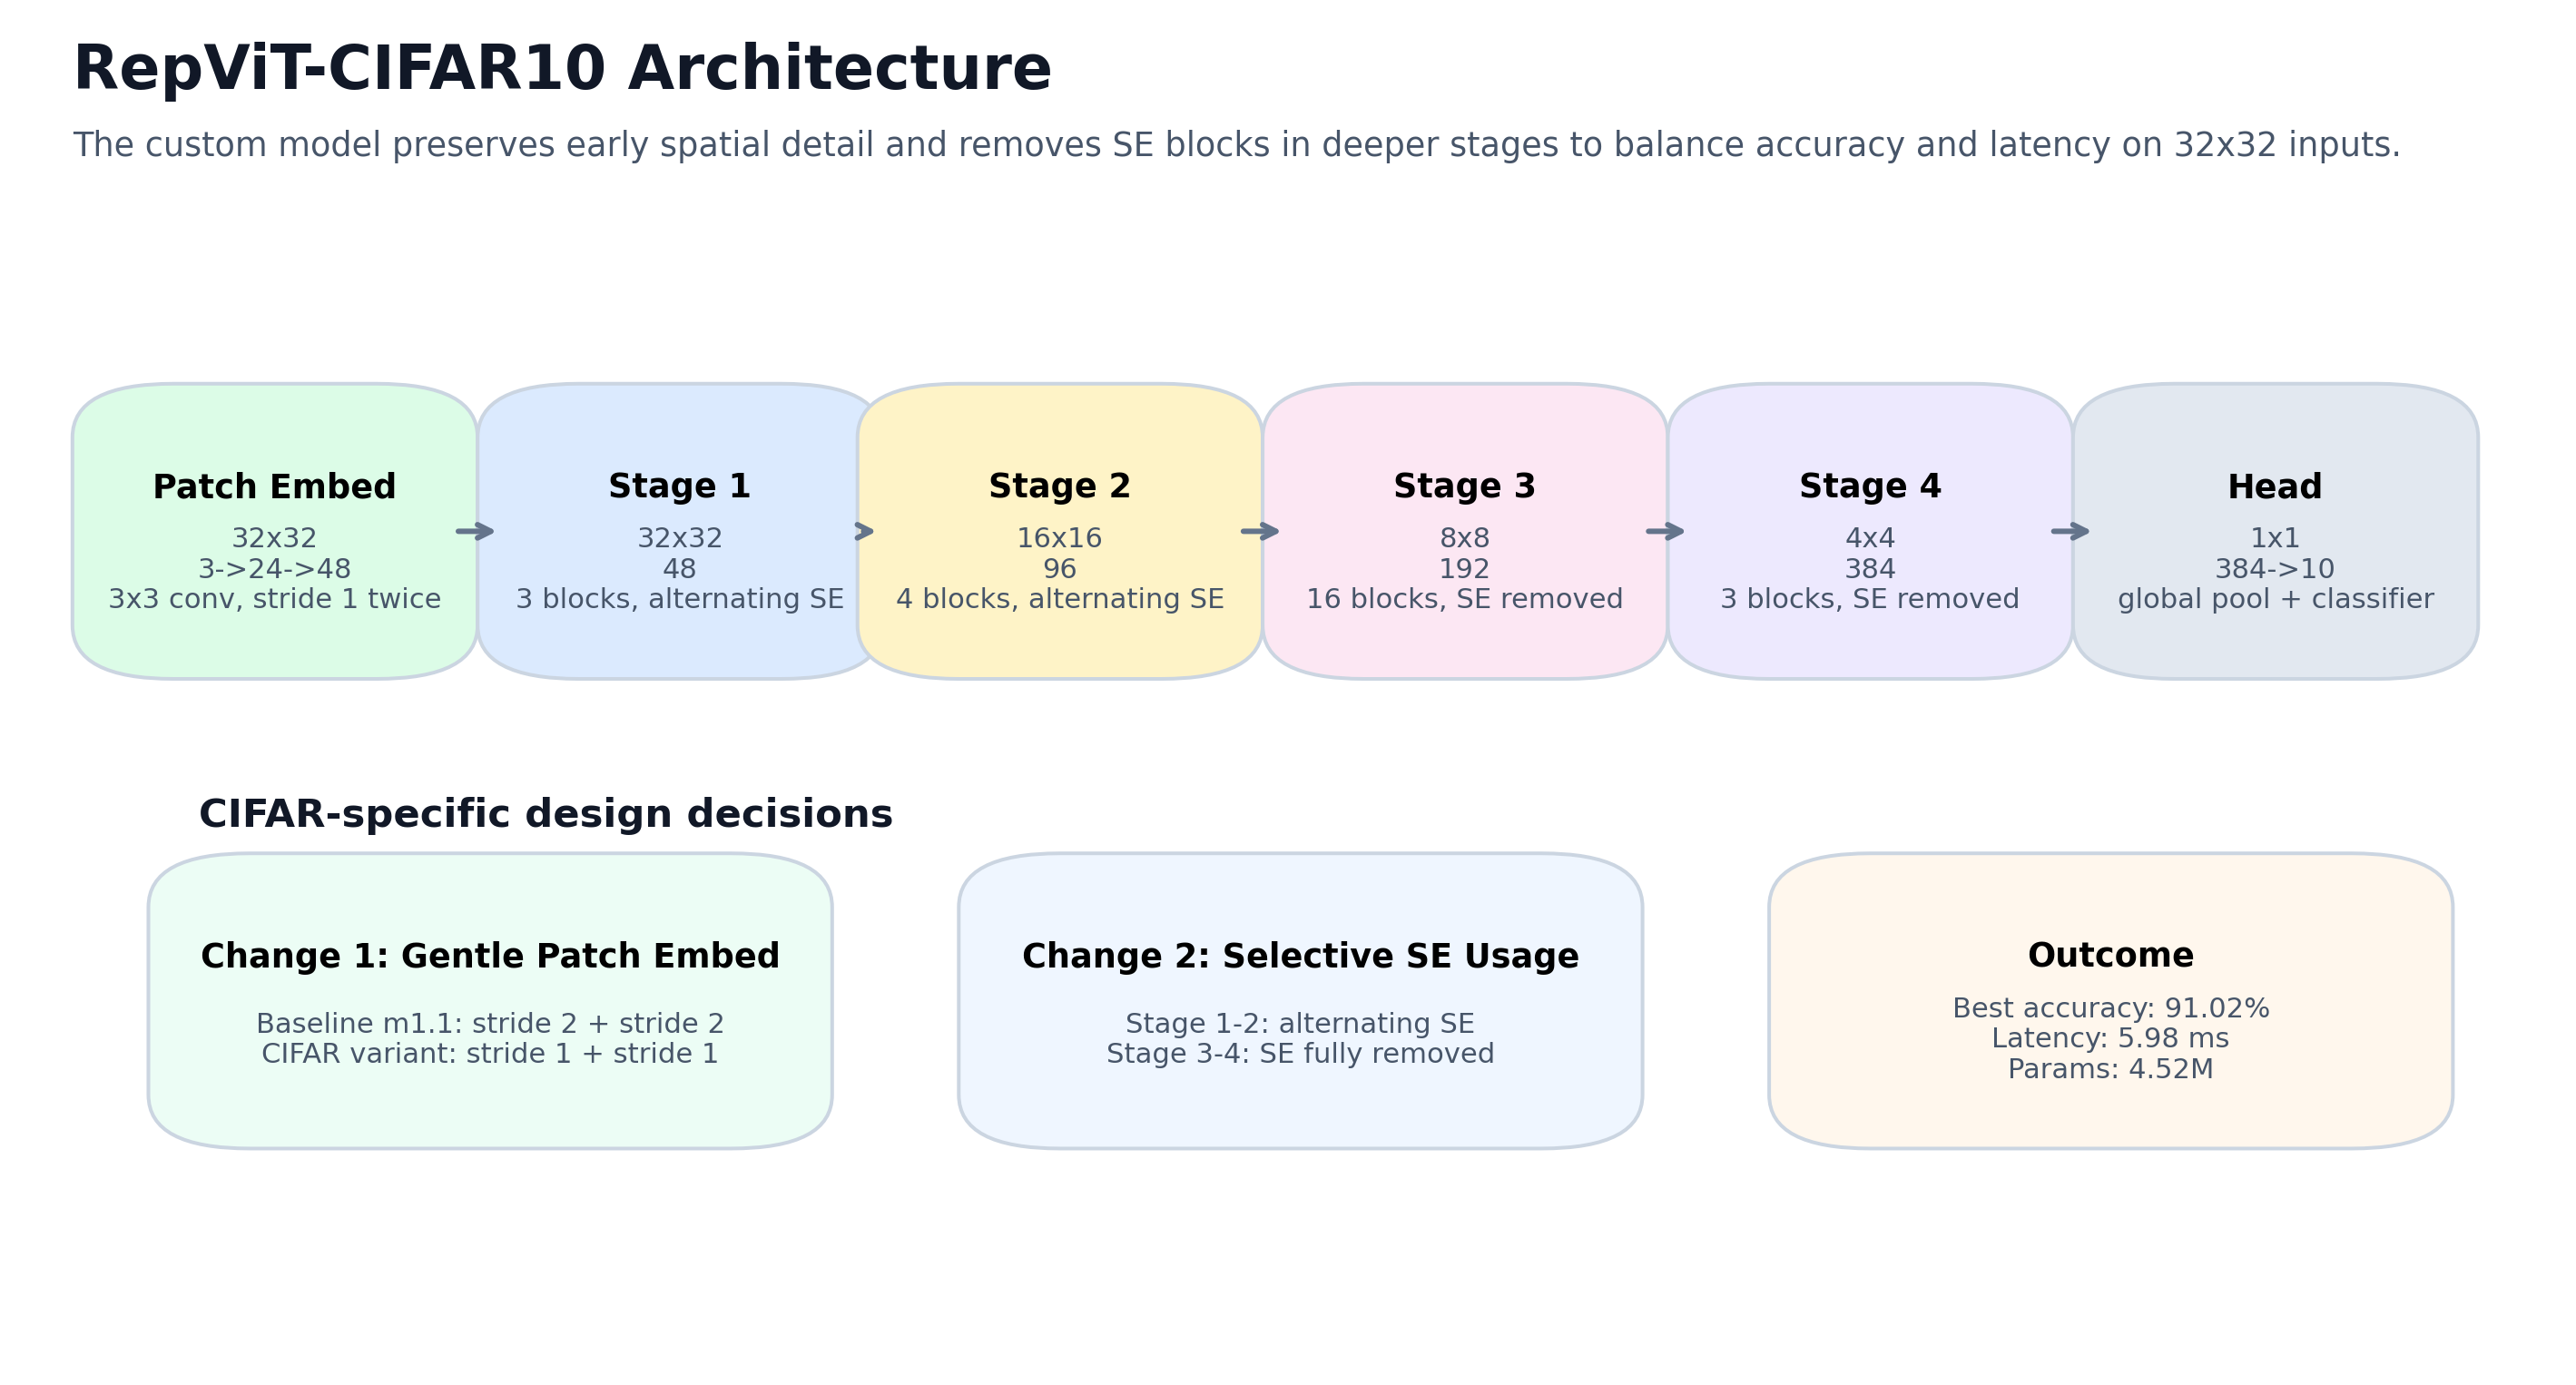
\includegraphics[width=\textwidth]{../visuals/repvit_cifar10_architecture.png}
    \caption{Overview of the CIFAR-specific RepViT architecture and the two main design modifications: gentler early downsampling and selective removal of SE blocks.}
    \label{fig:architecture}
\end{figure}

\section{Experimental Setup}

The training script uses the standard CIFAR-10 split with common image classification augmentations:
\begin{itemize}[leftmargin=1.5em]
    \item random crop with padding,
    \item random horizontal flip,
    \item normalization with CIFAR-10 channel statistics.
\end{itemize}

For the logged comparison runs, the script uses:
\begin{itemize}[leftmargin=1.5em]
    \item optimizer: AdamW,
    \item learning-rate schedule: cosine annealing,
    \item loss: cross entropy,
    \item batch size: 128,
    \item training length: 100 epochs in the archived log files used here.
\end{itemize}

Latency is measured using \texttt{measure\_latency.py} with:
\begin{itemize}[leftmargin=1.5em]
    \item batch size \(= 32\),
    \item 30 warm-up iterations,
    \item 200 timed runs,
    \item CUDA execution when available.
\end{itemize}

\begin{figure}[H]
    \centering
    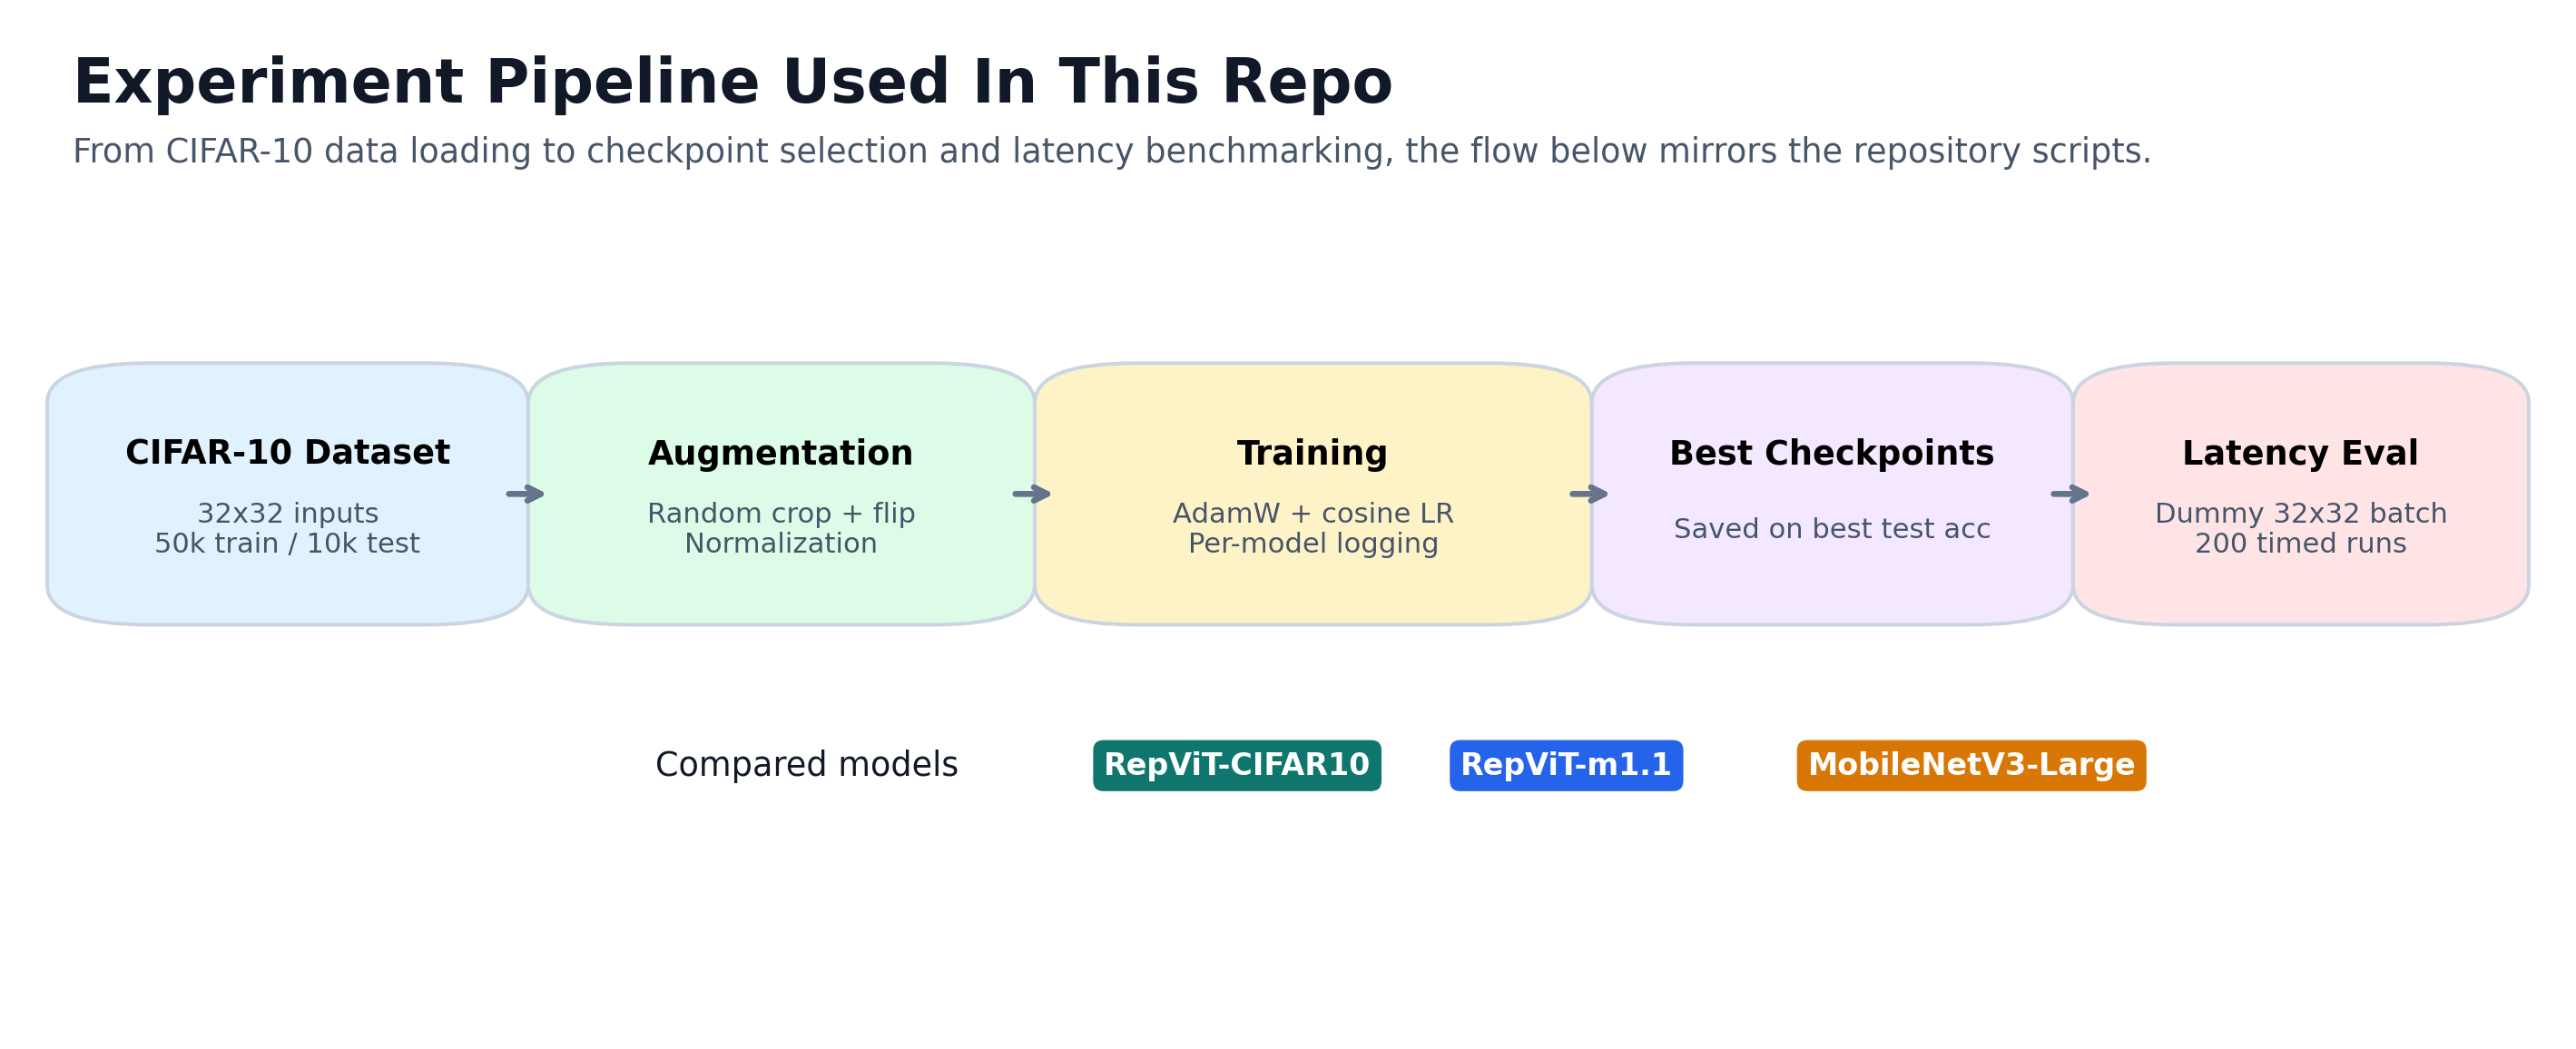
\includegraphics[width=\textwidth]{../visuals/experiment_pipeline.png}
    \caption{End-to-end experiment flow reflected in the repository scripts and generated assets.}
    \label{fig:pipeline}
\end{figure}

\section{Results}

\subsection{Quantitative Comparison}

\begin{table}[H]
    \centering
    \caption{Comparison of the three models using the repository's logged training and latency results.}
    \label{tab:results}
    \begin{tabular}{>{\raggedright\arraybackslash}p{4.0cm}cccc}
        \toprule
        Model & Best Test Acc. (\%) & Final Test Acc. (\%) & Latency (ms) & Params (M) \\
        \midrule
        RepViT-CIFAR10 & 91.02 & 90.75 & 5.98 & 4.52 \\
        RepViT-m1.1 & 87.39 & 87.39 & 5.95 & 7.78 \\
        MobileNetV3-Large & 75.77 & 75.77 & 2.98 & 4.21 \\
        \bottomrule
    \end{tabular}
\end{table}

The custom RepViT variant clearly outperforms the baseline RepViT-m1.1 in accuracy, improving best test accuracy by \(3.63\) percentage points. Importantly, this improvement does not come with a meaningful latency penalty: the logged latency difference between the two RepViT variants is only \(0.03\) ms, which is negligible in this context.

MobileNetV3-Large remains much faster, but the accuracy gap is large. Its lower latency therefore comes at a substantial cost in classification quality on this task.

\subsection{Training Dynamics}

\begin{figure}[H]
    \centering
    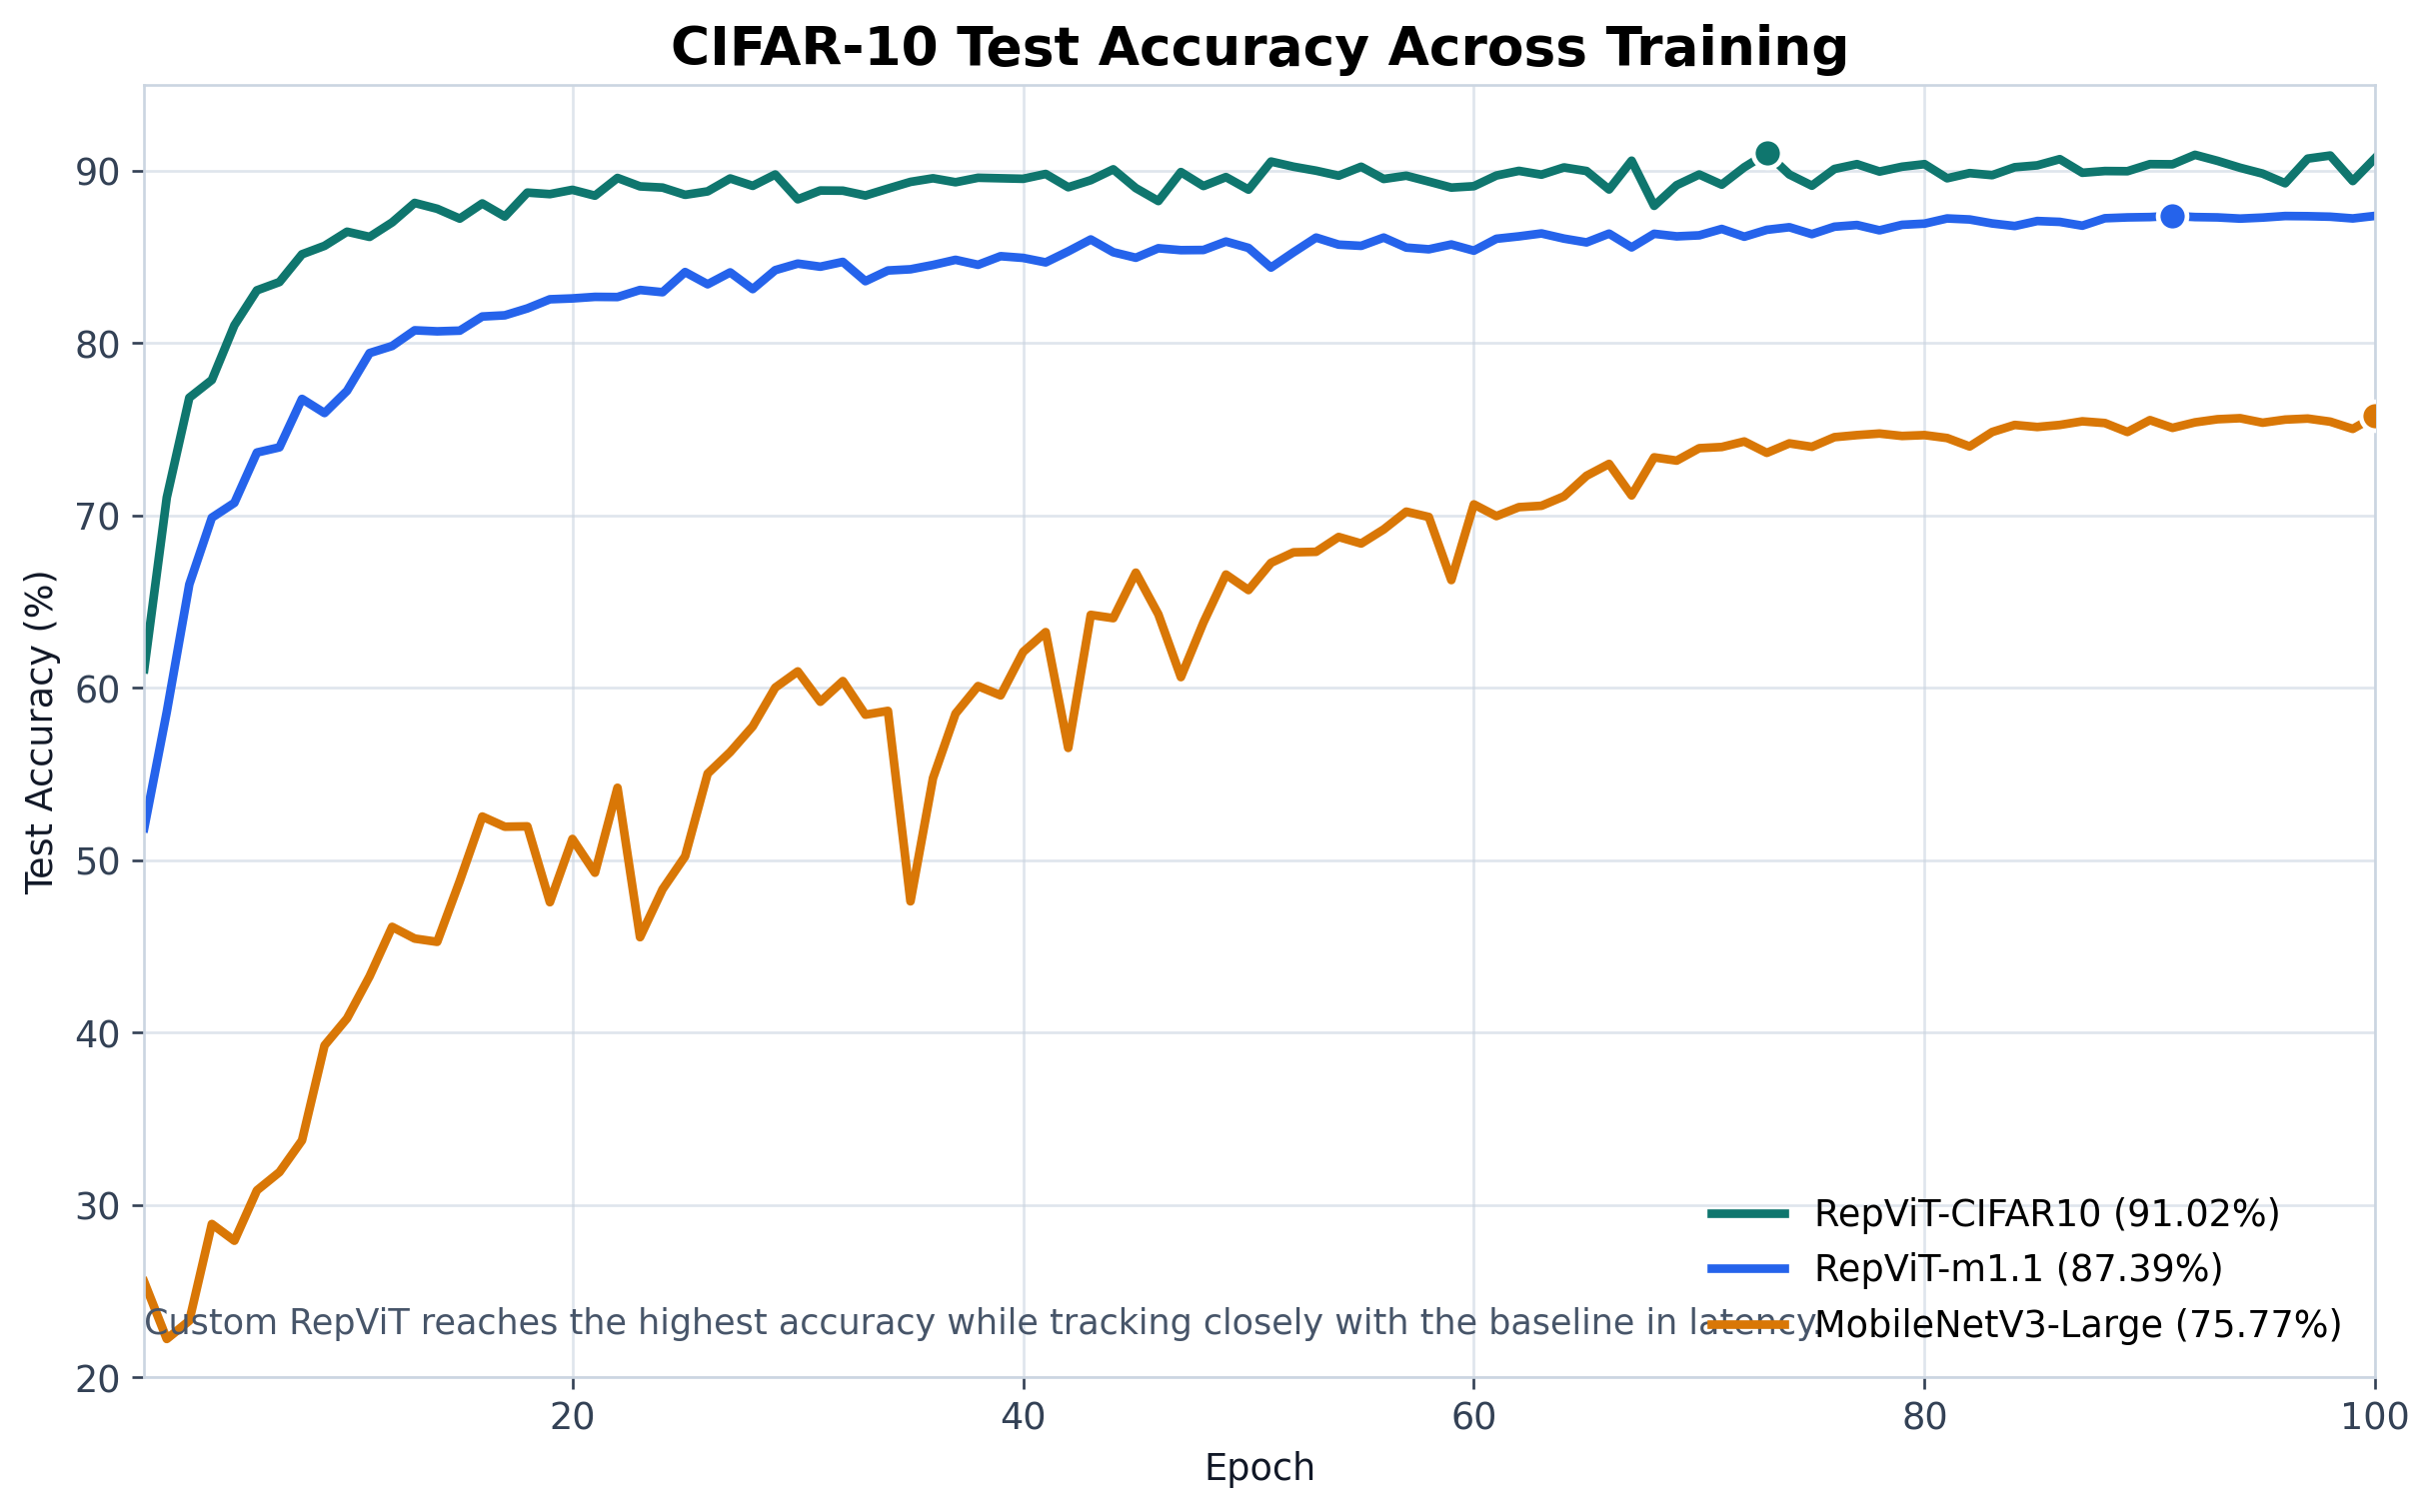
\includegraphics[width=\textwidth]{../visuals/training_curves.png}
    \caption{Test accuracy over training epochs for the three compared models.}
    \label{fig:training}
\end{figure}

The learning curves show several useful patterns:
\begin{itemize}[leftmargin=1.5em]
    \item RepViT-CIFAR10 converges quickly and consistently dominates the other two models through most of training.
    \item RepViT-m1.1 improves steadily but saturates well below the CIFAR-specific variant.
    \item MobileNetV3-Large learns more slowly and remains substantially less accurate throughout.
\end{itemize}

These dynamics support the architectural motivation. The stride reduction appears to help the model extract more useful features from small images early in training, while the selective SE design does not compromise convergence.

\subsection{Accuracy-Latency Trade-off}

\begin{figure}[H]
    \centering
    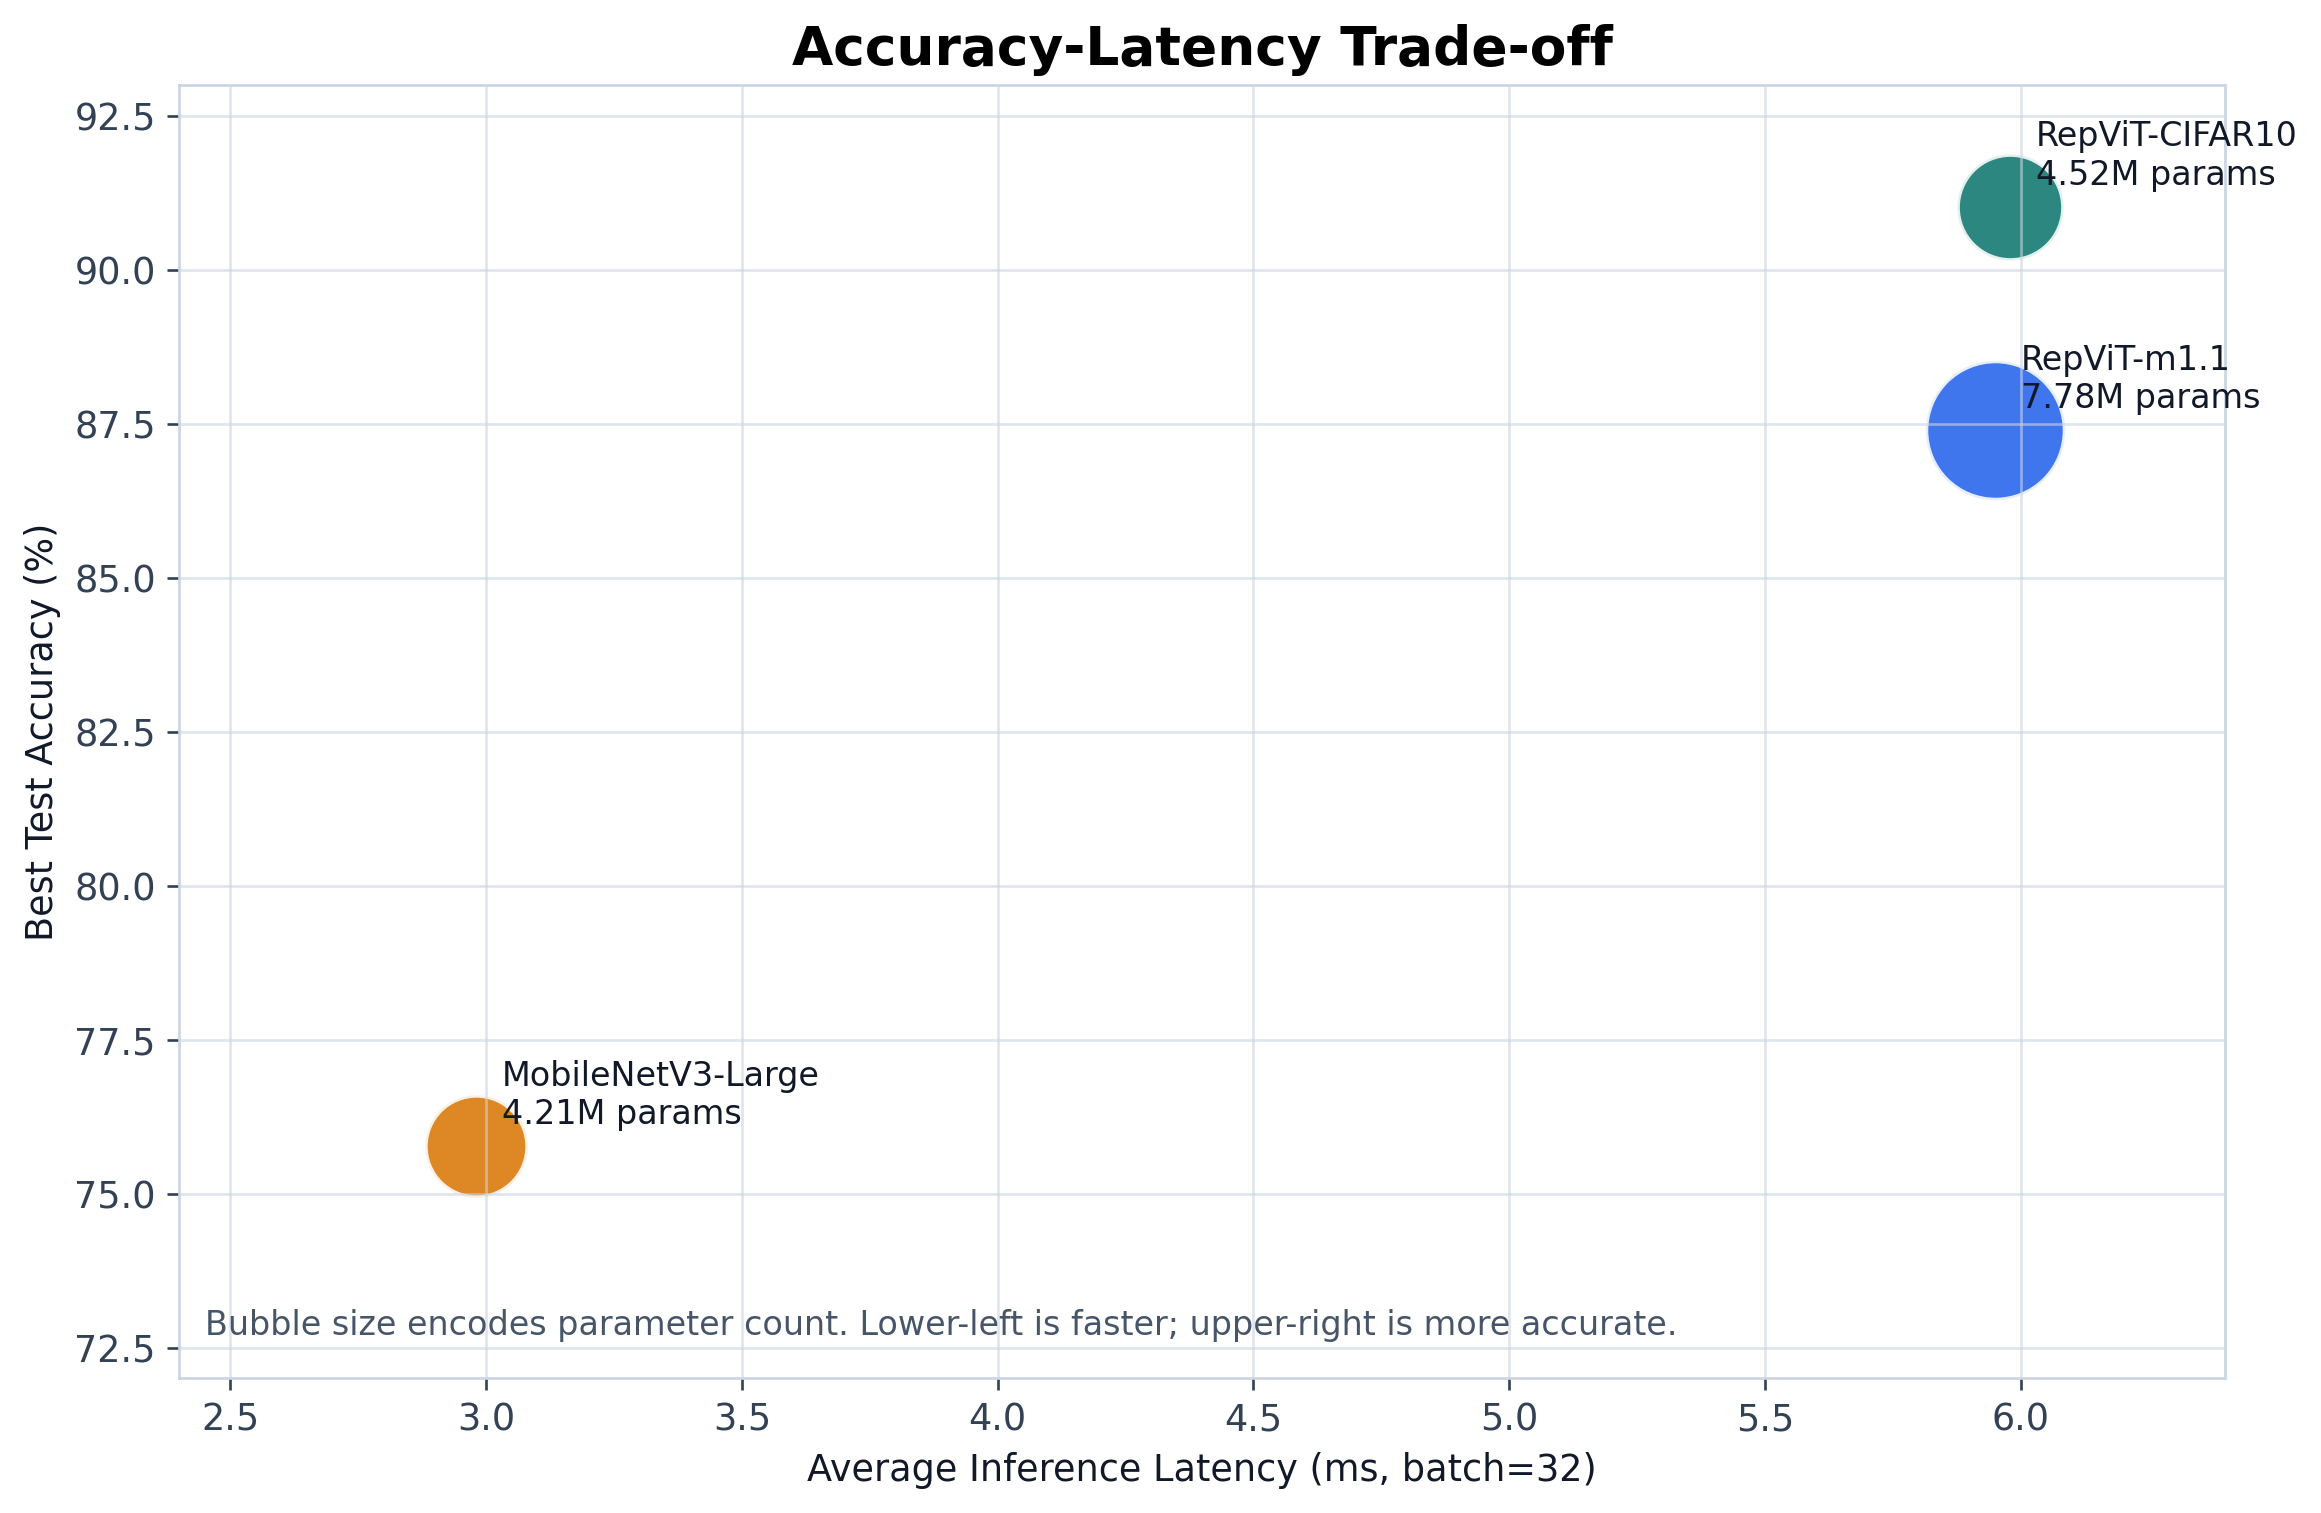
\includegraphics[width=0.92\textwidth]{../visuals/accuracy_latency_tradeoff.png}
    \caption{Accuracy-latency trade-off derived from the repository's measured inference logs. Bubble size represents parameter count.}
    \label{fig:tradeoff}
\end{figure}

The trade-off plot makes the design outcome especially clear:
\begin{itemize}[leftmargin=1.5em]
    \item the baseline RepViT-m1.1 and RepViT-CIFAR10 have nearly identical latency,
    \item the custom model reaches notably higher accuracy with fewer parameters,
    \item MobileNetV3-Large is best only if latency is the dominant objective and the project can tolerate a much lower accuracy ceiling.
\end{itemize}

\section{Discussion}

The modifications in this repository are well aligned with the properties of CIFAR-10.

\textbf{First, the stride reduction is strongly justified.} On \(32 \times 32\) inputs, aggressive early downsampling can remove exactly the sort of local structure that small-image classification depends on. Preserving resolution longer is therefore not a cosmetic change; it directly addresses a likely source of representational bottleneck.

\textbf{Second, the selective SE strategy is a practical latency-aware compromise.} The repository does not simply remove all SE blocks. Instead, it keeps them where they are most plausible to help, namely in the earlier stages where the network still has spatial richness and low-level detail to refine. It removes them where the computation is less likely to produce proportional gains. The resulting metrics suggest that this is a good trade for the task.

\textbf{Third, the final result is better than a naive ``smaller is faster'' story.} The custom model is not just more accurate than MobileNetV3; it is also more parameter-efficient than the baseline RepViT-m1.1 while achieving higher accuracy at nearly the same latency. That indicates the gains come from architectural fit to the dataset, not simply from adding capacity.

\section{Limitations}

The report should be read with several practical limitations in mind:
\begin{itemize}[leftmargin=1.5em]
    \item latency results depend on the hardware and CUDA environment used for measurement,
    \item no confusion matrix or per-class breakdown is available in the repository logs,
    \item the current comparison uses a single logged setup rather than repeated runs with confidence intervals,
    \item the automation script still advertises 30 epochs, while the saved logs used here reflect 100 epochs.
\end{itemize}

These limitations do not invalidate the conclusions, but they do frame them as engineering evidence from this codebase rather than a fully controlled benchmark study.

\section{Conclusion}

This repository presents a sensible and effective adaptation of RepViT for CIFAR-10. The architectural motivation is clear:
\begin{itemize}[leftmargin=1.5em]
    \item reduce early stride because CIFAR-10 images are small and cannot afford aggressive spatial collapse,
    \item retain some SE capacity early because channel recalibration still helps when feature maps preserve detail,
    \item remove deeper SE blocks to hold latency in check once the representation has already become compact.
\end{itemize}

The measured outcome supports these decisions. RepViT-CIFAR10 reaches the best observed accuracy in the repository while keeping inference latency essentially unchanged relative to the baseline RepViT-m1.1. For this project, the modifications are not only intuitive but empirically justified.

\section*{Appendix: Source Files Used}

This report is based on the implementation and logs in:
\begin{itemize}[leftmargin=1.5em]
    \item \texttt{README.md}
    \item \texttt{model/repvit.py}
    \item \texttt{train\_cifar10.py}
    \item \texttt{measure\_latency.py}
    \item \texttt{repvit\_cifar10\_cifar10\_training.log}
    \item \texttt{repvit\_m1\_1\_cifar10\_training.log}
    \item \texttt{mobilenetv3\_large\_100\_cifar10\_training.log}
    \item \texttt{repvit\_cifar10\_latency.log}
    \item \texttt{repvit\_m1\_1\_latency.log}
    \item \texttt{mobilenetv3\_large\_100\_latency.log}
\end{itemize}

\end{document}
